% One hydra step at n=2. The cut head is rust. Two new copies of the shortened branch appear.
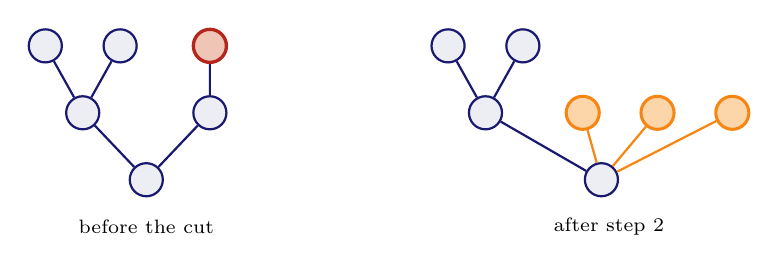
\begin{tikzpicture}[x=0.95cm,y=0.85cm,
  v/.style={circle,draw=MidnightBlue,thick,fill=MidnightBlue!8,inner sep=0pt,minimum size=4.2mm},
  head/.style={circle,draw=BrickRed,line width=1.2pt,fill=BrickRed!20,inner sep=0pt,minimum size=4.2mm},
  copy/.style={circle,draw=BurntOrange,line width=1.1pt,fill=BurntOrange!30,inner sep=0pt,minimum size=4.2mm}]
  % before
  \node[v] (r) at (0,0) {};
  \node[v] (a) at (-0.85,1) {};
  \node[v] (b) at (0.85,1) {};
  \node[v] (c) at (-1.35,2) {};
  \node[v] (d) at (-0.35,2) {};
  \node[head] (e) at (0.85,2) {};
  \draw[MidnightBlue,thick] (r)--(a) (r)--(b) (a)--(c) (a)--(d) (b)--(e);
  \node[font=\scriptsize] at (0,-0.7) {before the cut};
  % after
  \begin{scope}[xshift=5.4cm]
    \node[v] (r2) at (0.4,0) {};
    \node[v] (a2) at (-1.15,1) {};
    \node[copy] (b2) at (0.15,1) {};
    \node[copy] (b3) at (1.15,1) {};
    \node[copy] (b4) at (2.15,1) {};
    \node[v] (c2) at (-1.65,2) {};
    \node[v] (d2) at (-0.65,2) {};
    \draw[MidnightBlue,thick] (r2)--(a2) (a2)--(c2) (a2)--(d2);
    \draw[BurntOrange,thick] (r2)--(b2) (r2)--(b3) (r2)--(b4);
    \node[font=\scriptsize] at (0.5,-0.7) {after step $2$};
  \end{scope}
\end{tikzpicture}
